\section{EppaBasic-ympäristö}
Tässä luvussa kerrotaan EppaBasic-ympäristöstä
eli käyttöliittymästä ja ohjelmointikielestä.
Aluksi kuitenkin kerrotaan ympäristölle
asetetuista tavoitteista.
\fxnote{Laajenna tai poista}

\subsection{Tavoitteet}
EppaBasicin tärkein tavoite on olla
mahdollisimman helppo oppia,
mutta samalla mahdollistaa
monipuolisten ohjelmien toteuttamisen.
Yksinkertaiset ja helpot grafiikkakomennot ovat tärkeitä,
sillä moni aloitteleva (ja miksei myös kokenutkin)
ohjelmoija haluaa nähdä työnsä tulokset.
Varsinkin aloittelijoille ohjelman aukeaminen
viime vuosituhannelta tuttuun komentokehotteen
voi olla hyvinkin epätyydyttävää.
\fxnote{Media computation}
\fxnote{Vika virke paremmin}

Toinen EppaBasicin tärkeä tavoite on olla
mahdollisimman helposti käyttöönotettava,
sillä usein uutta ohjelmointikieltä opetellessa
kuluu useita tunteja jo pelkän
ohjelmointiympäristön asentamiseen.
Ympäristön asentamiseksi usein
tätyy asentaa erikseen koodin
kirjoittamiseen käytettävä ohjelma
ja koodia ymmärtävä kääntäjä,
sekä määrittää asetukset oikein.
Lisäksi koodin jakaminen
voi olla hankalaa. Monissa kouluissa
ongelmia saattaa lisäksi aiheuttaa byrokratia,
joka vaikeuttaa uusien ohjelmistojen asentamista
koulun tietokoneille.
EppaBasic onkin toteutettu
selaimessa toimivaksi, joten
käyttöönottaminen onnistuu
helposti navigoimalla osoitteeseen
\url{http://eppabasic.fi}.

Ennen projektin aloittamista pohdimme,
täyttäisikö jokin olemassa oleva
kieli jo nämä tavoitteet.
Kuitenkin miettiessämme vaihtoehtoja
useat kielet olivat joko vanhentuneita,
niiden asentaminen tai oppiminen on hankalaa,
tai niillä grafiikan tekeminen on työlästä.
Tämän takia päädyimme uuden kielen tekemiseen.
Ohjelmointikielten luominen on lisäksi hauskaa
ja opettavaista.

\subsection{Käyttöliittymä}
EppaBasic-ympäristö koostuu kahdesta osasta,
joista ensimmäisenä esittelen ohjelmakoodin
kirjoittamiseen käytettävän käyttöliittymän.

\begin{figure}[h]
    \centering
    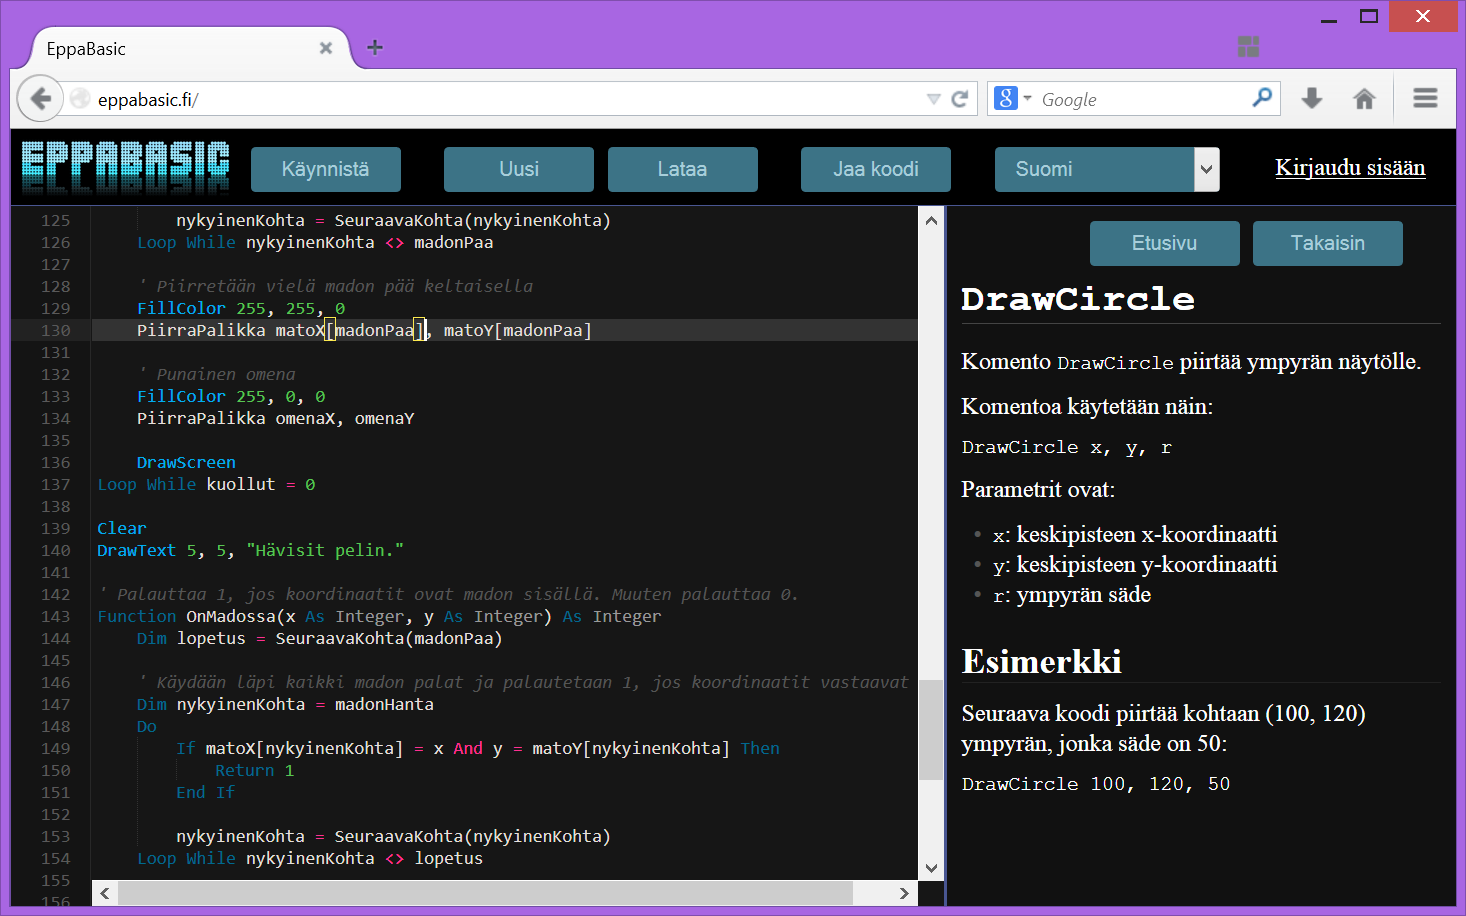
\includegraphics[width=1\textwidth]{kayttoliittyma}
    \caption{EppaBasicin käyttöliittymä. Ylhäällä työkalupalkki, vasemmalla koodimuokkain ja oikealla käyttöohje.}
    \label{img:kayttoliittyma}
\end{figure}

EppaBasicin käyttöliittymä on toteutettu
kokonaan käyttäen HTML:ää ja JavaScriptiä.
Näin on saatu aikaan kaikissa moderneissa
selaimissa toimiva yhtenäinen käyttöliittymä.

EppaBasicin käyttöliittymä tarjoaa kaikki
ohjelmointiin tarvittavat toiminnot.
Yläpalkissa on koodin suorittamisen käynnistävä
nappi sekä napit koodin tallentamiseen ja lataamiseen.
Lisäksi koodin voi jakaa muille linkin avulla.
Kirjautumalla sisään koodin voi tallentaa
omalle käyttäjälleen, jolloin se on käytettävissä
kaikilla tietokoneilla.

Käyttöliittymän vasemmalla reunalla on
suuri koodimuokkain, johon suoritettava
ohjelmakoodi kirjoitetaan.
Koodimuokkaimen oikealla puolella on
käyttöohje, jossa on kaikille
EppaBasicin tarjoamille funktioille
ja toiminnoille ohje esimerkkeineen.

EppaBasicin käyttämä tekstinmuokkain mahdollistaa
virheiden ilmoittamisen käyttäjälle jo
koodia kirjoitettaessa.
Näin käyttäjä saa heti palautetta tekemistään
virheistä ja voi korjata ne saman tien.
Jos käyttäjä ei huomaa virheen syytä,
hän voi lukea virheen sisältämän
kuvauksen virheestään omalla kielellään
(ks. Kuva \ref{img:virhe}).

\begin{figure}[h]
    \centering
    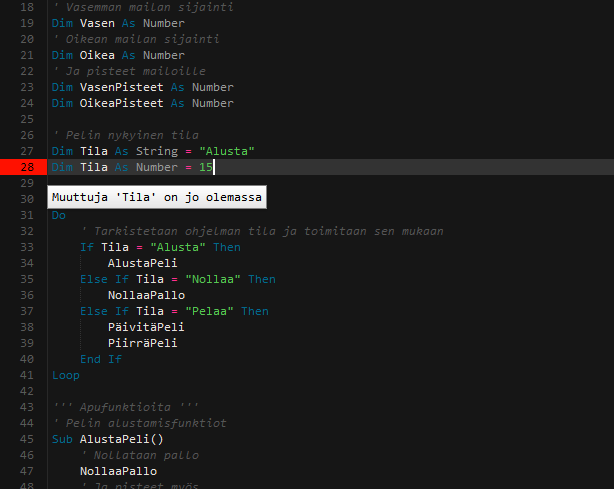
\includegraphics[width=0.5\textwidth]{virhe}
    \caption{EppaBasicin koodimuokkain, jossa näkyy käyttäjän tekemä virhe sekä virheen selitys.}
    \label{img:virhe}
\end{figure}

\subsection{Kieli}
EppaBasicin-ympäristön toinen osa on
itse ohjelmointikieli.
Ohjelmointikieli tukee
muuttujia,
ehto- ja toistorakenteita,
matemaattisten lausekkeiden laskemista,
funktioita,
merkkijonoja,
taulukoita sekä
omien funktioiden
ja aliohjelmien luomista.
EppaBasicissa on myös
laaja standardikirjasto,
jossa on matematiikka-,
merkkijono-, syöte- ja
grafiikkakomentoja.

EppaBasicin avulla voi helposti
piirtää yksinkertaisia geometrisiä
muotoja (ks. Koodi \ref{code:geometria}).
Muotojen värin vaihtaminen
onnistuu myös helposti.

Heittomerkin \eb{'} jälkeinen
teksti rivillä on kommenttia,
jota EppaBasic ei suorita.
Kommentit on tarkoitettu
työkaluksi ohjelmoijalle
koodin selkeyttämiseen.

\codeandimage{geometria}{Geometriaesimerkki}{code:geometria}

EppaBasicissa on yksinkertainen
\eb{For}-toistorakenne, jonka
avulla voi suorittaa saman
koodin monta kertaa.
Toistettava koodi alkaa
\eb{For}-avainsanaa seuraavalta
riviltä ja loppuu ennen riviä,
jolla on \eb{Next}-avainsana.
\eb{For}-rakenteen sisällä voi
käyttää toistorakenteessa määriteltyä
muuttujaa, jonka arvo käy läpi
kaikki luvut annetulla välillä
(ks. Koodi \ref{code:for-geometria}).

\codeandimage{for-geometria}{Geometriaa \eb{For}-rakenteella}{code:for-geometria}

\eb{For}-toistorakennetta voi
käyttää myös matemaattisten 
ongelmien ratkausemiseen
(ks. Koodi \ref{code:for-summa}).

\codeandimage{for-summa}{Ohjelma, joka laskee summan $1^2+2^2+3^2+...+100^2$.}{code:for-summa}

EppaBasicia voi käyttää myös
kokonaisten pelien luomiseen.
Tästä esimerkkinä toimii
kielellä tehty moninpelattava
pong-peli
(ks. Kuva \ref{img:pong} ja Liite \ref{app:pong}),
jota voi kokeilla myös
EppaBasicin sivustolla.

\begin{figure}[h]
    \centering
    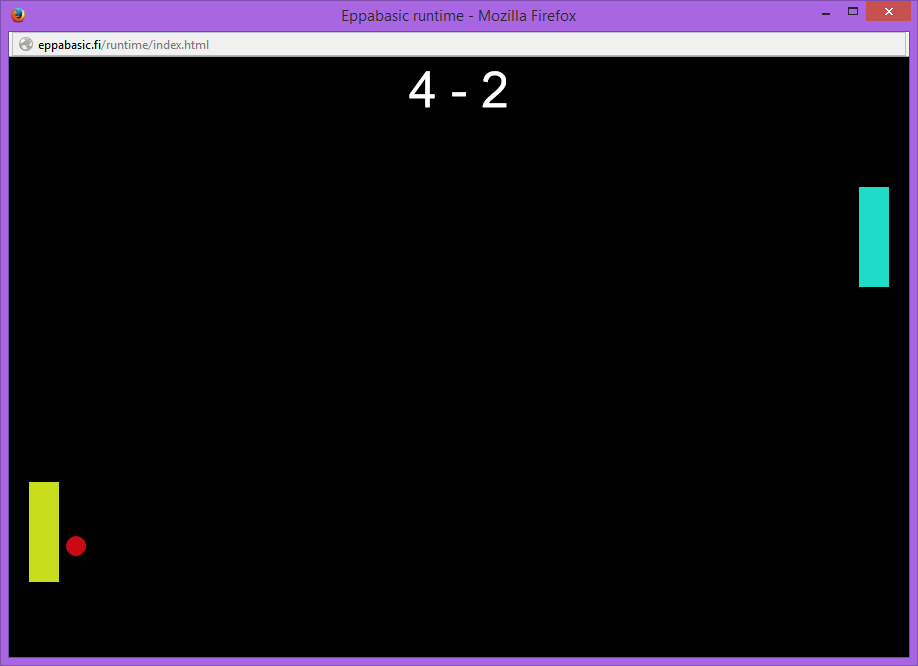
\includegraphics[width=0.5\textwidth]{pong}
    \caption{EppaBasicilla toteutettu kahdenpelattava pong-peli.}
    \label{img:pong}
\end{figure}